\chapter{Results} \label{study_results}

This Chapter describes all the results gathered throughout the study. They are presented accordingly to the method used and for each one of them I reported the raw numbers and relevance with respect to the RQs.

As a final note, due to confidentiality issues it was not possible to report the raw data. For this reason, as briefly explained in the previous Chapter, all the sensitive information has been eliminated and anonymized.



\section{Informal Interviews}
As mentioned in the Data Gathering section the informal interviews conducted within this study helped to narrow the scope of the study itself and to gain knowledge of important problems faced by testers along the time frame of this study.

Furthermore, given the randomness associated with this method I will only report the topics covered in such conversations. Moreover, due to confidentiality and anonymity, I am not allowed to report most of the literal quotations that are of interest for this study.

The topics covered, during such interviews are reported in Table \ref{tab:informal_interviews_topics}. For completeness's sake I also included the date and the approximate length of these conversations.

		\begin{table}[htb]
			\centering
			%\renewcommand{\arraystretch}{1.2}
			\caption{Topics covered while performing the Informal interviews}
			\label{tab:informal_interviews_topics}
			\begin{tabulary}{\columnwidth}{|L|L|L|}
				\hline
				
				\textbf{Date} {\tiny (YYYY/MM/DD)} & \textbf{Approx. duration} & \textbf{Topics covered} \\
				\hline
				
				2015/02/13 &
				10 min. &
				- How does the test pipeline works.\newline
				- Recurrent problems with high level tests. \\
				\hline
				
				2015/02/16 &
				10 min. &
				- Strategy with smoke UFT tests. \newline
				- Strategy with test automation in general. \\
				\hline
				
				2015/02/19 &
				10 min. &
				- Approach of different teams to testing. \\
				\hline
				
				2015/02/23 &
				5 min. &
				- Different Definitions of Done in use. \\
				\hline
				
				2015/02/24 &
				10 min. &
				- Strategy with regression testing. \newline
				- How issues with system level testing are reported. \\
				\hline
				
				2015/02/27 &
				10 min. &h
				- How the automation works (Jenkins, Nightly builds etc.\ ). \\
				\hline
				
				
                
			\end{tabulary}		
		\end{table}


\section{Mining of the Forum}
The process explained in Section \ref{mining_forum} yielded 15 possible interesting documents. Those are in various formats, spacing from actual entries in the forum to pictures of whiteboards taken during workshops.

Some of these documents are central to this study, whereas others only highlight problems that are platform or tool specific. For transparency's sake I also reported these entries, but they were not used in the \textit{theory generation} step.

\begin{table}[htb]
	\centering
	%\renewcommand{\arraystretch}{1.2}
	\caption{Number of hits in Confluence for a given keyword}
	\label{tab:confluenceMiningResults}
	\begin{tabulary}{\textwidth}{|L|L|L|L|}
		\hline
		\textbf{Keyword} & 
		\textbf{Total hits} &
		\textbf{After First Filter} &
		\textbf{After Second Filter}\\ \hline
		
		\textit{"test mainteneance"} &
		28 &
		18 &
		9 \\ \hline
		
		\textit{"tests strategy"} &
		297 &
		138 &
		11 \\ \hline
		
		\textit{"test refactoring"} &
		13 &
		3 &
		3 \\ \hline
		
		\textit{"test quality"} &
		36 &
		4 &
		4 \\ \hline
		

	\end{tabulary}		
\end{table}

\begin{figure}[ht]
    \centering
    \begin{minipage}[t]{0.45\linewidth}
        \centering
        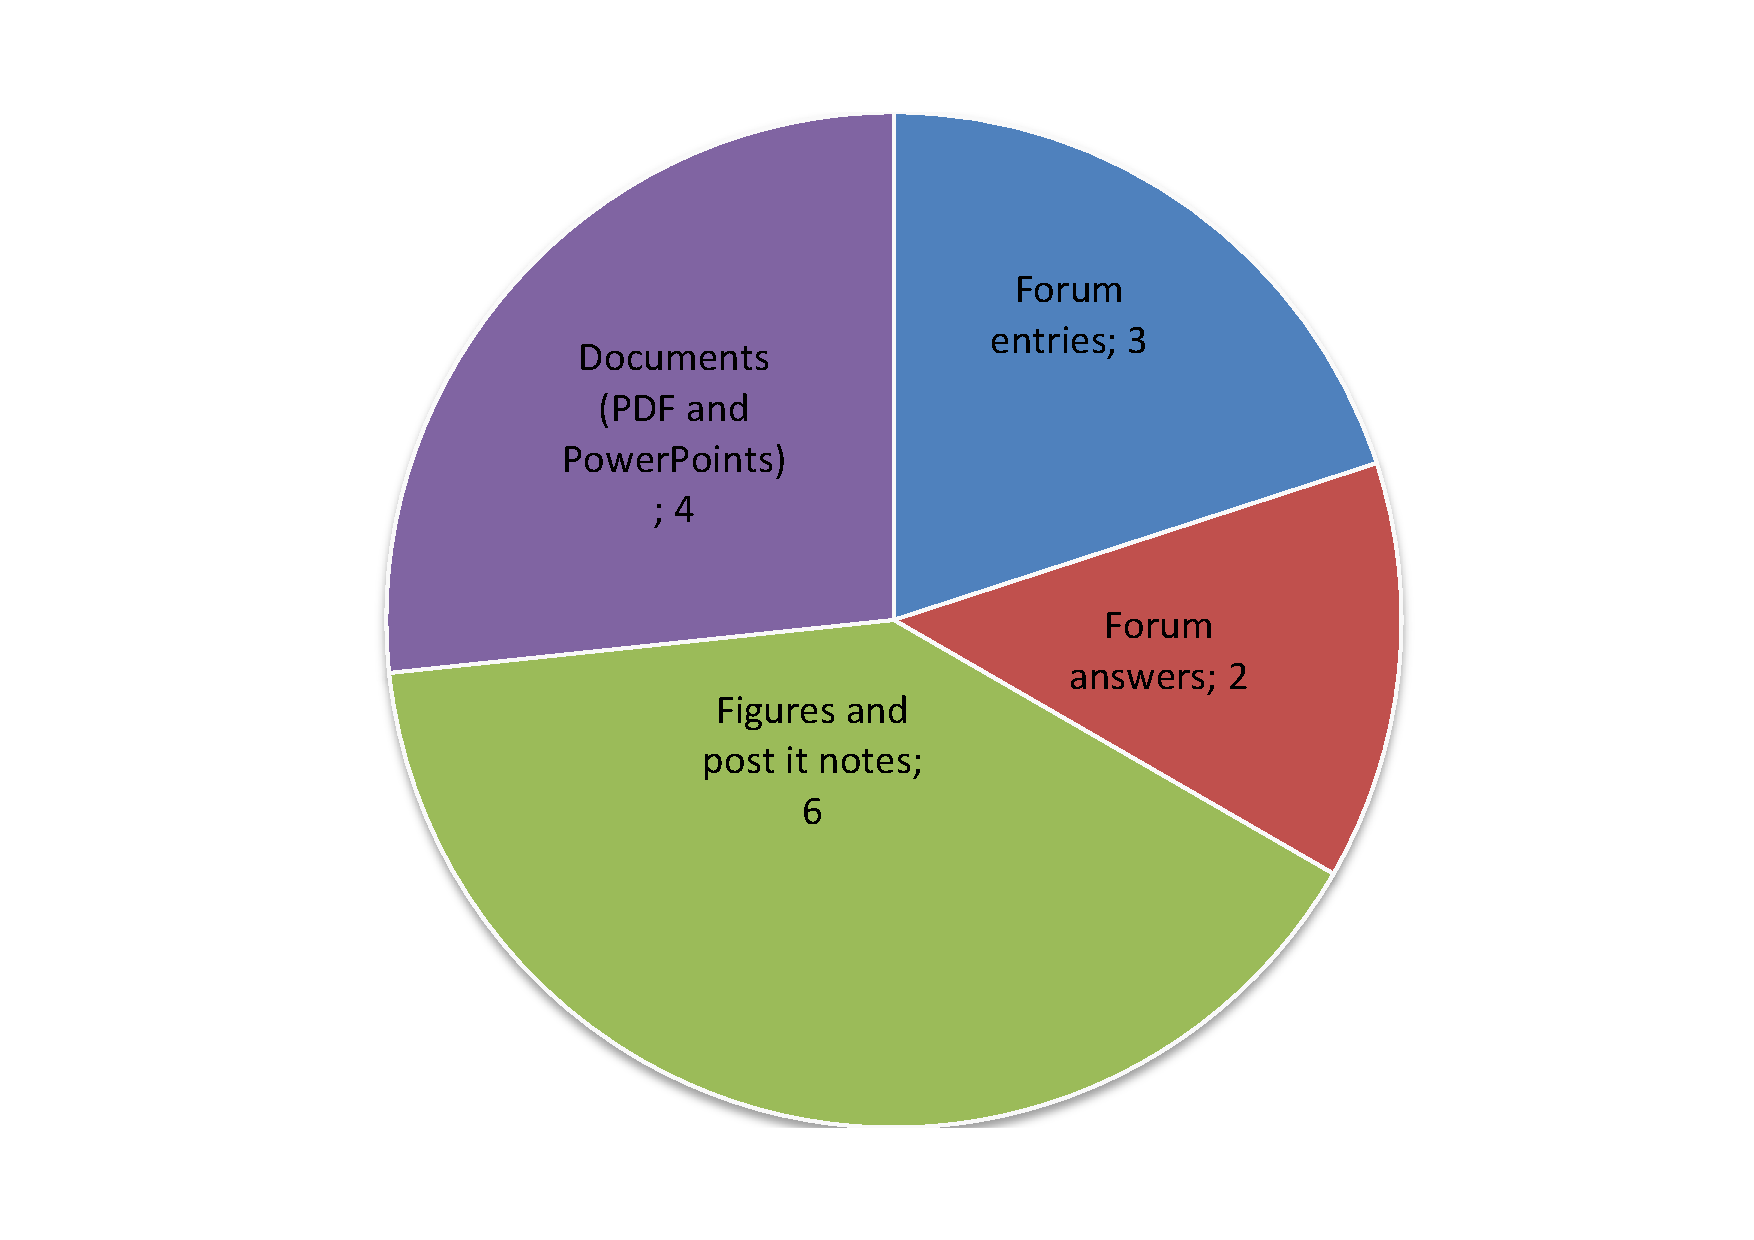
\includegraphics[width=\textwidth]{figure/results/confluence_doc_types}
        \caption{Type of the results yielded by the forum's mining}
        \label{fig:confluence_types}
    \end{minipage}
    \hspace{0.5cm}
    \begin{minipage}[t]{0.45\linewidth}
        \centering
        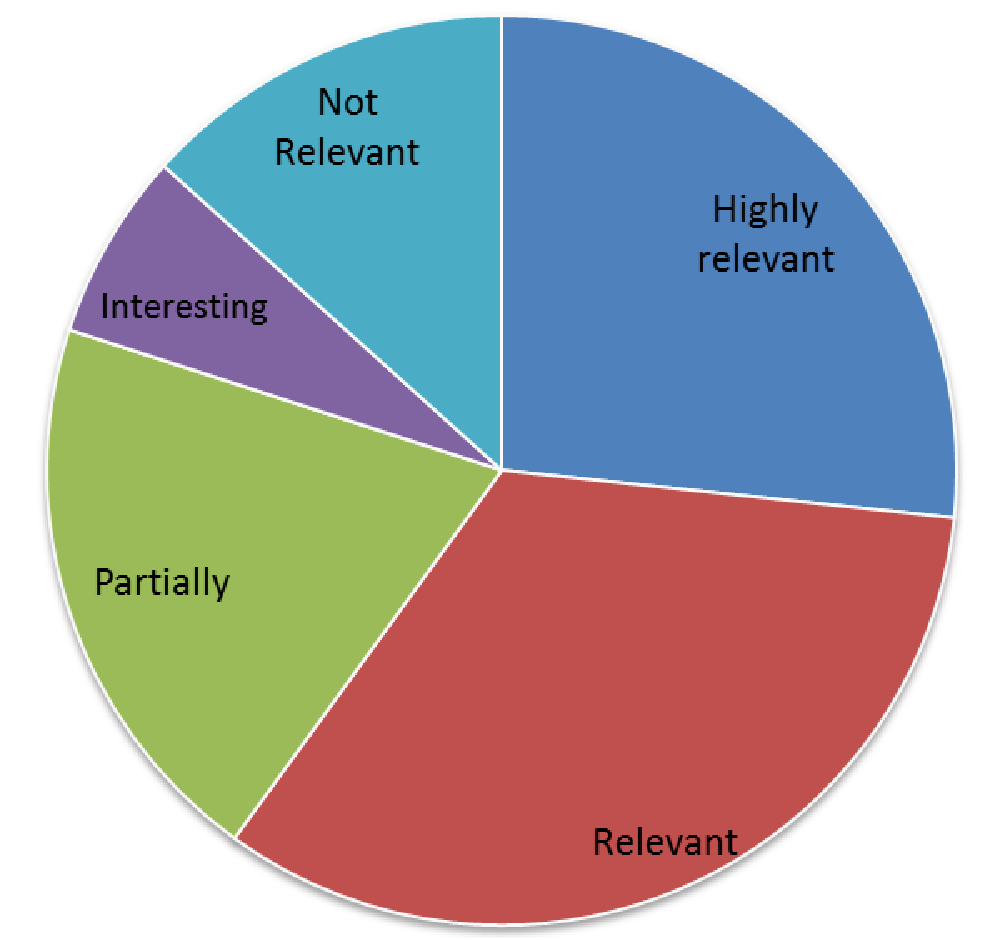
\includegraphics[width=\textwidth]{figure/results/confluence_doc_relevance}
        \caption{Relevance of Confluence entries according to the RQs defined in this study}
        \label{fig:confluence_relevance}
    \end{minipage}
\end{figure}


\section{Mining of the Issue Tracer / Backlogs}

\todo{Update method description for issue tracker analysis.}

The process described in Section \ref{mining_issue_tracker}, as of the 11th of April 2015, yielded a total of 104 entries which has been inspected accordingly. For each issue several factors has been considered.

Firstly, issues that entailed CUD operations (create, update, and delete) on the testware source code has been separated from the ones reporting environments' problem. This task however, is not trivial due to a thin boundary between the two categories. For instance, an issue attributed to the environment can be instead triggered by problems within the source code. Among the one belonging to the first group, the results of interest are the ones revealing maintenance activities, i.e.\ update and delete.

From such subset further statistics have been collected. Namely, story point and time statistics which reflect how long the issue has been opened without been addressed and how long did it take to address it.

\todo{Fine tune the script for mining the result}

\todo{Plot the chart from this data.}

\todo{Check if a time analysis of issues related to particular projects yields something interesting}

\section{Analysis of the Repositories}

\section{Semi-Structured Interviews}